%%% user_manual.tex ---

%% Author: Nicolas Niclausse
%% Version: $Id$

\def\RCS$#1: #2 ${\expandafter\def\csname RCS#1\endcsname{#2}}
\RCS$Revision$
\RCS$Date$

\documentclass{IDXDOC-en}
\usepackage{shortcuts}

% --------------------------------------------
% Title
% --------------------------------------------
\doctitle{Tsung User's manual}

%\addauthor{Nicolas}{Niclausse}{nicolas.niclausse@niclux.org}

\doccopyright{Nicolas Niclausse.}
\docversion{\RCSRevision}
\docreldate{\RCSDate}
\docref{tsung-user-manual}

\begin{document}
\maketitle
\newpage
\tableofcontents

\section{Introduction}

\subsection{What is Tsung ?}

\program{Tsung} (formerly IDX-Tsunami) is a distributed load testing tool. It is
protocol-independent and can currently be used to stress HTTP, WebDAV, SOAP,
PostgreSQL, MySQL, LDAP, and Jabber/XMPP servers.

It is distributed under the GNU General Public License version 2.


\subsection{What is Erlang and why is it important for Tsung ?}

\program{Tsung's} main strength is its ability to simulate a huge number of
simultaneous user from a single CPU. When used on cluster you can
generate a really impressive load on a server with a modest cluster,
easy to set-up and to maintain.

\program{Tsung} is developed in Erlang and this is where the power
of \program{Tsung} resides.

\par Erlang is a \emph{concurrency-oriented} programming language.
Tsung is based on the Erlang OTP (Open Transaction Platform) and
inherits several characteristics from Erlang:

\begin{itemize}
\item \emph{Performance}: Erlang has been made to support hundred thousands
of lightweight processes in a single virtual machine.
\item \emph{Scalability}: Erlang runtime environment is naturally
distributed, promoting the idea of process's location transparency.
\item \emph{Fault-tolerance}:Erlang has been built to develop robust,
fault-tolerant systems. As such, wrong answer sent from the server
to \program{Tsung} does not make the whole running benchmark crash.
\end{itemize}

More informations on Erlang on \url{http://www.erlang.org} and
\url{http://www.erlang-projects.org/}


\subsection{Tsung background}

History:
\begin{itemize}
\item \program{Tsung} development was started by Nicolas Niclausse in
  2001 as a distributed jabber load stress tool for internal use at
  \url{http://IDEALX.com/}.  It has evolved as an open-source
  multi-protocol load testing tool several months later. The HTTP
  support was added in 2003, and this tool has been used for several
  industrial projects.  It is now hosted by Erlang-projects, and
  supported by \url{http://process-one.net/}. The list of contributors
  is available in the source archive
  (\url{https://svn.process-one.net/tsung/trunk/CONTRIBUTORS}).

\item It is an industrial strength implementation of a \emph{stochastic model}
for real users simulation. User events distribution is based on a
Poisson Process. More information on this topic in:

Z. Liu, N. Niclausse, et C. Jalpa-Villanueva.  \strong{Traffic Model
  and Performance Evaluation of Web Servers}. \emph{Performance Evaluation,
Volume 46, Issue 2-3, October 2001}.

\item This model has already been tested in the INRIA \emph{WAGON}
  research prototype (Web trAffic GeneratOr and beNchmark). WAGON was
  used in the \url{http://www.vthd.org/} project (Very High Broadband
  IP/WDM test platform for new generation Internet applications, 2000-2004).

\end{itemize}

\program{Tsung} has been used for very high load tests:

\begin{itemize}
\item \emph{Jabber/XMPP} protocol:
  \begin{itemize}
  \item 90 000 simultaneous jabber users on a
  4-node Tsung cluster (3xSun V240 + 1 Sun V440)
\item 10 000 simultaneous users.
  \program{Tsung} was running on a 3-computers cluster (CPU
  800Mhz)
  \end{itemize}
\item \emph{HTTP and HTTPS} protocol:
  \begin{itemize}
  \item 12 000 simultaneous users.
  \program{Tsung} were running on a 4-computers cluster. The
  tested platform reached 3 000 requests per second.
  \end{itemize}
\end{itemize}

\program{Tsung} has been used  at:

\begin{itemize}
\item \emph{DGI} (Direction Générale des impôts): French finance ministry
\item \emph{Cap Gemini Ernst \& Young}
\item \emph{IFP} (Institut Français du Pétrole): French Research Organization
for Petroleum
\item \emph{LibertySurf}
\item Sun\texttrademark for their Mooddlerooms platform on Niagara processors:
 \url{http://blogs.sun.com/kevinr/resource/Moodle-Sun-RA.pdf}
\end{itemize}


\section{Features}

\subsection{Tsung main features}

\begin{itemize}
\item \emph{High Performance}: \program{Tsung} can simulate a
  huge number of simultaneous users per physical computer: It can
  simulates thousands of users on a single CPU (Note: a simulated user
  is not always active: it can be idle during a \varname{thinktime}
  period). Traditional injection tools can hardly go further than a
  few hundreds (Hint: if all you want to do is requesting a single URL
  in a loop, use \program{ab}; but if you want to build complex
  scenarios with extended reports, \program{Tsung} is for you).
\item \emph{Distributed}: the load can be distributed on a cluster of
client machines
\item \emph{Multi-Protocols} using a plug-in system: HTTP (both standard
web traffic and SOAP),  Webdav, Jabber/XMPP and PostgreSQL are currently
supported. Experimental LDAP and MySQL plugins were included in the 1.3.0 release.
\item \emph{SSL} support
\item \emph{Several IP addresses} can be used on a single machine using
the underlying OS IP Aliasing
\item \emph{OS monitoring} (CPU, memory and network traffic) using Erlang
agents on remote servers or \emph{SNMP}
\item \emph{XML configuration system}: complex user's scenarios are written
  in XML. Scenarios can be written with a simple browser using the
  Tsung recorder (HTTP and PostgreSQL only).
\item \emph{Dynamic scenarios}: You can get dynamic data from the
  server under load (without writing any code) and re-inject it in
  subsequent requests. You can also loop, restart or stop a
  session when a string (or regexp) matches the server response.
\item \emph{Mixed behaviours}: several sessions can be used to simulate
different type of users during the same benchmark. You can define
the proportion of the various behaviours in the benchmark scenario.
\item \emph{Stochastic processes}: in order to generate a realistic traffic,
user thinktimes and the arrival rate can be randomize using a probability
distribution (currently exponential)
\end{itemize}

\subsection{HTTP related features}

\begin{itemize}
\item HTTP/1.0 and HTTP/1.1 support
\item GET, POST, PUT, DELETE and HEAD requests
\item Cookies: Automatic cookies management
\item \verb|'|GET If-modified since\verb|'| type of request
\item WWW-authentication Basic
\item User Agent support
\item Any HTTP Headers can be added
\item Proxy mode to record sessions using a Web browser
\item SOAP support using the HTTP mode (the SOAPAction HTTP header is
  handled).
\item HTTP server or proxy server load testing.
\end{itemize}

\subsection{WEBDAV related features}

The Webdav plugin is a superset of the HTTP plugin. It adds the
following features:

\begin{itemize}
\item Methods implemented: DELETE, CONNECT, PROPFIND, PROPPATCH, COPY,
  MOVE, LOCK, UNLOCK, MKCOL, REPORT, OPTIONS
\item Recording of DEPTH, IF, TIMEOUT OVERWRITE, DESTINATION, URL and
  LOCK-TOKEN Headers.
\end{itemize}

\subsection{Jabber/XMPP related features}

\begin{itemize}
\item Authentication (plain-text, digest and sip-digest)
\item presence and register messages
\item Chat messages to online or offline users
\item Roster set and get requests
\item Global users\verb|'| synchronization can be set on specific actions
\item raw XML messages
\end{itemize}

\subsection{PostgreSQL related features}

\begin{itemize}
\item Basic and MD5 Authentication
\item Basic Queries (Extended queries not yet supported)
\item Proxy mode to record sessions
\end{itemize}

\subsection{MySQL related features}
This plugin is experimental. It works only with MySQL version 4.1 and higher.
\begin{itemize}
\item Secured Authentication method only (MySQL >= 4.1)
\item Basic Queries
\end{itemize}

\subsection{LDAP related features}
This plugin is experimental.

\begin{itemize}
\item bind
\item add, modify and search queries
\item starttls (only with R12B-0 Erlang and up)
\end{itemize}

\subsection{Complete reports set}

Measures and statistics produced by Tsung are extremely feature-full.
They are all represented as a graphic. \program{Tsung} produces
statistics regarding:

\begin{itemize}
\item \emph{Performance}: response time, connection time,  decomposition of the user scenario based on request grouping  instruction (called \textit{transactions}), requests per second
\item \emph{Errors}: Statistics on page return code to trace errors
\item \emph{Target server behaviour}: An Erlang agent can gather information
from the target server(s). Tsung produces graphs for CPU and memory
consumption and network traffic. SNMP is also supported.
\end{itemize}
\par Note that \program{Tsung} takes care of the synchronization process
by itself. Gathered statistics are «synchronized».

 It is possible to generate graphs during the benchmark as statistics
are gathered in real-time.

\subsection{Highlights}

\program{Tsung} has several advantages over other injection tools:


\begin{itemize}
\item \emph{High performance} and \emph{distributed benchmark}: You
  can use Tsung to simulate tens of thousands of virtual users.
\item \emph{Ease of use}: The hard work is already done for all supported
protocol. No need to write complex scripts. Dynamic scenarios only
requires small trivial piece of code.
\item \emph{Multi-protocol support}: \program{Tsung} is for example one of
the only tool to benchmark SOAP applications
\item \emph{Monitoring} of the target server(s) to analyze the behaviour
and find bottlenecks. For example, it has been used to analyze cluster
symmetry (is the load properly balanced ?) and to determine the best
combination of machines on the three cluster tiers (Web engine, EJB
engine and database)
\end{itemize}



\section{Installation}

This package has been tested on Linux, FreeBSD and Solaris. It should
work on Erlang supported platforms (Linux, Solaris, *BSD, Win32 and
MacOS-X).

\subsection{Dependencies}
\begin{itemize}
\item Erlang/OTP R10B-0 and up
  (\url{http://www.erlang.org/download.html}). Erlang is now
  part of fedora and debian repository.
  \item extended regexp module (used for dynamic variables):
    gregexp.erl available at
    \url{http://www.cellicium.com/erlang/contribs/} . The module is
    included in the source and binary distribution of \program{Tsung}. It
    is released under the EPL License.
  \item pgsql module made by Christian Sunesson (for the PostgreSQL plugin):
    sources available at
    \url{http://jungerl.sourceforge.net/} . The module is
    included in the source and binary distribution of \program{Tsung}. It
    is released under the EPL License.
  \item mysql module made by Magnus Ahltorp \& Fredrik Thulin  (for the mysql plugin):
    sources available at
    \url{http://www.stacken.kth.se/projekt/yxa/} . The modified module is
    included in the source and binary distribution of \program{Tsung}. It
    is released under the three-clause BSD License.
  \item eldap module  (for the LDAP plugin):
    sources available at
    \url{http://jungerl.sourceforge.net/} . The module is
    included in the source and binary distribution of \program{Tsung}. It
    is released under the GPL License.
  \item mochiweb libs (for xpath parsing, optionally used for dynamic variables in
    the HTTP plugin):
    sources available at
    \url{http://code.google.com/p/mochiweb/} . The module is
    included in the source and binary distribution of \program{Tsung}. It
    is released under the MIT License.
   \item  gnuplot and perl5 (optional; for graphical output with
    \command{tsung\_stats.pl} script).  The Template Toolkit is used for HTML
    reports (see \url{http://template-toolkit.org/})
  \item for distributed tests, you need an ssh access to remote
    machines without password (use a RSA/DSA key without pass-phrase or
    ssh-agent) (rsh is also supported)
\item bash
\end{itemize}
\subsection{Compilation}

\begin{Verbatim}
./configure
 make
 make install
\end{Verbatim}
\subsection{Configuration}

The default configuration file is \file{~/.tsung/tsung.xml} (
there are several sample files in
\file{/usr/share/doc/tsung/examples}).

Log files are saved in \file{~/.tsung/log/} . A new sub-directory
is created for each test using the current date as name
(\file{~/.tsung/log/20040217-09:40} for ex.)

\subsection{Feedback}

Use the Tsung mailing list (see
\url{https://lists.process-one.net/mailman/listinfo/tsung-users}) if you have
suggestions or questions about \program{Tsung}. You can also use the
bugtracker available at \url{https://support.process-one.net/browse/TSUN}.

\section{Benchmark approach}

\subsection{HTTP/WebDAV benchmark approach}

\subsubsection{Benchmarking a Web server}

\begin{enumerate}
\item Record one or more sessions: start the recorder with: \command{tsung
    recorder}, and then configure your browser to use Tsung
  proxy recorder (the listen port is 8090). A session file will be
  created. For HTTPS recording, use \userinput{http://ssl-} instead of
    \userinput{https://} in your browser.
\item Edit / organize scenario, by adding recorded sessions in the
  configuration file.
\item Write small code for dynamic parts if needed and place dynamic mark-up
in the scenario.
\item Test and adjust scenario to have a nice progression of the load. This
is highly dependent of the application and of the size of the target
server(s). Calculate the normal duration of the scenario and use the
interarrival time between users and the duration of the phase to estimate
the number of simultaneous users for each given phase.
\item Launch benchmark with your first application parameters set-up:
  \command{tsung start}
\item Wait for the end of the test or stop by hand with
  \command{tsung stop} (reports can also be generated during the
  test (see § \ref{sec:statistics-reports}) : the statistics are
  updated every 10 seconds). For a brief summary of the current
  activity, use \command{tsung status}
\item Analyze results, change parameters and relaunch another benchmark
\end{enumerate}

\subsubsection{WEBDAV }

It's the same approach as HTTP: first you start to record one or more
sessions with the recorder:
\command{tsung -p webdav  recorder}

\subsubsection{Benchmarking a proxy server}

By default, the HTTP plugin is used to benchmark HTTP servers. But you
can also benchmark HTTP Proxy servers. To do that, you must add in the
\varname{options} section:

\begin{Verbatim}
  <option type="ts_http" name="http_use_server_as_proxy" value="true"></option>
\end{Verbatim}


\subsection{LDAP benchmark approach}

An LDAP plugin for the recorder is not yet implemented, so you have to
write the session by yourself; see section \ref{sec:session:ldap} for
more information.

\subsection{PostgreSQL benchmark approach}

It's the same approach as HTTP: first you start to record one or more
sessions with the recorder:
\command{tsung -p pgsql  recorder}

This will start a proxy listening to port 8090 and will proxy requests
to 127.0.0.0:5432.

To choose another port and/or address:
\command{tsung -L 5432 -I 10.6.1.1 -P 5433 -p pgsql  recorder}

This will start a proxy listening to port 5432 and will proxy requests
to 10.6.1.1:5433.

\subsection{MySQL benchmark approach}

A MySQL plugin for the recorder is not yet implemented, so you have to
write the session by yourself; see section \ref{sec:session:mysql} for
more information.

\subsection{Jabber/XMPP benchmark approach}

\subsubsection{Overview}

This paragraph explains how to write a session for Jabber/XMPP.

There are two differences between HTTP and Jabber testing:
\begin{enumerate}
\item There is no recorder for Jabber, so you have to write your
  sessions by hand (an example is provided in
  \ref{sec:sessions:jabber}).
\item the jabber plugin does not parse XML; instead it uses packet
  acknowledgments.
\end{enumerate}



There is no recorder for Jabber, so you have to write your sessions by
hand (an example is provided in \ref{sec:sessions:jabber}).

\subsubsection{Acknowledgments of messages}

Since the jabber plugin does not parse XML (historically, it was for
performance reasons), you must have a way to tell when a request is
finished. There are 3 possibilities:

\begin{description}
 \item[ack=local] as soon as a packet is received from the server, the
request is considered as completed. Hence if you use a local ack with a request
that do not require a response from the server (presence for ex.), it
 will wait forever (or until a timeout is reached).
 \item[ack=no\_ack] as soon as the request is send, it is considered as completed (do
not wait for incoming data)
 \item[ack=global] synchronized users. its main use is for waiting for all
users to connect before sending messages. To do that, set a request
with global ack (it can be the first presence msg:

\begin{Verbatim}
   <request> <jabber type="presence" ack="global"/> </request>
\end{Verbatim}
)

You also have to specify the number of users to be connected:

\begin{Verbatim}
<option type="ts_jabber" name="global_number" value="100"></option>
\end{Verbatim}

To be sure that exactly \varname{global\_number} users are started, add the
\userinput{'maxnumber'} attribute to \varname{'users'}

\begin{Verbatim}
    <users maxnumber="100" interarrival="1.0" unit="second"></users>
\end{Verbatim}

If you do not specify \varname{maxnumber}, the global ack will be reset every
\varname{global\_number} users
\end{description}

\label{bidi:presence}
\strong{New in 1.2.2:} This version adds an new option for a
session. if you set the attribute \varname{bidi} (for bidirectional)
in the \varname{session} tag: \userinput{<session ... bidi='true'>},
then incoming messages from the server will be analyzed. Currently,
only roster subscription requests are handled: if a user received a
subscription request (\userinput{<presence ... type='subscribe'>}), it
will respond with a \userinput{<presence ... type='subscribed'>}
message.

\subsubsection{Status: Offline, Connected and Online}

You can send messages to offline or online users. A user is considered
online when he has send a \userinput{presence:initial} message (before
this message , the state of the user is \varname{connected}).

If you want to switch back to \varname{connected} before going
\varname{offline}, you can use a \userinput{presence:final} message:

\userinput{presence:final} does two things:
\begin{enumerate}
\item It removes the client from the list of Online users, and moves
  them into the list of Connected users.
\item  It sends a broadcast presence update of type='unavailable'.
\end{enumerate}

\userinput{presence:final} is optional.

\emph{warn:} this is new in \strong{1.2.0}, in earlier version, only 2
status were available: online and offline; a user was considered
online as soon as it was connected.

\subsubsection{Authentication}

Below are configuration examples for the possible authentication
methods.  Note: the regular expressions used here are only examples -
they may need to be altered depending on how a particular server
implementation composes messages (see also ~\ref{sec:jabber-options}
for password settings).


\begin{itemize}
\item \strong{plain authentication} - sends clear-text passwords:
\begin{Verbatim}
  <session probability="100" name="jabber-plain" type="ts_jabber">

    <request> <jabber type="connect" ack="local"></jabber> </request>

    <thinktime value="2"></thinktime>

    <transaction name="auth_plain">
      <request> <jabber type="auth_get" ack="local"></jabber> </request>
      <request> <jabber type="auth_set_plain" ack="local"></jabber> </request>
    </transaction>
    ...
  </session>
\end{Verbatim}
\item \strong{digest authentication}  as described in XMPP JEP-0078: Non-SASL Authentication
   \url{http://www.jabber.org/jeps/jep-0078.html}
\begin{Verbatim}
  <session probability="100" name="jabber-digest" type="ts_jabber">

    <!-- regexp captures stream ID returned by server -->
    <request>
      <dyn_variable name="sid" regexp="&lt;stream:stream id=&quot;\(.*\)&quot; xmlns:stream"/>
      <jabber type="connect" ack="local"></jabber>
    </request>

    <thinktime value="2"></thinktime>

    <transaction name="auth_digest">
      <request> <jabber type="auth_get" ack="local"></jabber> </request>
      <request subst='true'> <jabber type="auth_set_digest" ack="local"></jabber> </request>
    </transaction>
    ...
  </session>
\end{Verbatim}
\item \strong{sip-digest authentication}
\begin{Verbatim}
  <session probability="100" name="jabber-sipdigest" type="ts_jabber">

    <request> <jabber type="connect" ack="local"></jabber> </request>

    <thinktime value="2"></thinktime>

    <transaction name="auth_sipdigest">
      <!-- regexp captures nonce value returned by server -->
      <request>
        <dyn_variable name="nonce"
          regexp="&lt;Nonce encoding=&quot;hex&quot;&gt;\(.*\)&lt;\/Nonce&gt;"/>
        <jabber type="auth_get" ack="local"></jabber>
      </request>
      <request subst='true'> <jabber type="auth_set_sip" ack="local"></jabber> </request>
    </transaction>
    ...
  </session>
\end{Verbatim}
\end{itemize}

\section{Using the proxy recorder}


The recorder has three plugins: for HTTP, WebDAV and for PostgreSQL.

To start it, run \command{tsung -p <PLUGIN> recorder}, where \varname{PLUGIN} can be
\userinput{http}, \userinput{webdav} or  \userinput{pgsql} for PostgreSQL. The default plugin is \userinput{http}.


The proxy is listening to port 8090. You can change the port with
\userinput{-L portnumber}.

To stop it, use \command{tsung stop\_recorder}.

The recorded session is created as
\file{~/.tsung/tsung_recorderYYYMMDD-HH:MM.xml}; if it doesn't work,
take a look at \file{~/.tsung/log/tsung.log-tsung_recorder@hostname}

During the recording, you can add custom tag in the XML file, this can
be useful to set transactions or comments:
\command{tsung record\_tag "<transaction name='login'>''}

Once a session has been created, you can insert it in your main configuration
file, either by editing by hand the file, or by using an ENTITY
declaration, like:

\begin{Verbatim}
<!DOCTYPE tsung SYSTEM "/usr/share/tsung/tsung-1.0.dtd" [
 <!ENTITY mysession1 SYSTEM "/home/nniclausse/.tsung/tsung_recorder20051217-13:11.xml">
]>
...
<sessions>
  &mysession1;
</sessions>
\end{Verbatim}

\subsection{PostgreSQL}

For PostgreSQL, the proxy will connect to the server at IP 127.0.0.1
and port 5432. Use \userinput{-I serverIP} to change the IP and
\userinput{-P portnumber} to change the port.

\subsection{HTTP and WEBDAV}

For HTTPS recording, use \userinput{http://ssl-} instead of
\userinput{https://} in your browser

\strong{New in 1.2.2:}: For HTTP, you can configure the recorder to
use a parent proxy (but this will not work for https). Add the -u
option to enable parent proxy, and use \userinput{-I serverIP} to set
the IP and \userinput{-P portnumber} to set the port of the parent.




\section{Understanding tsung.xml configuration file}

The default encoding is utf-8.  You can use a different encoding, like in:

 \begin{Verbatim}
<?xml version="1.0" encoding="ISO-8859-1"?>
 \end{Verbatim}

\subsection{File structure}

 Scenarios are enclosed into Tsung tags:

 \begin{Verbatim}
<?xml version="1.0"?>
<!DOCTYPE tsung SYSTEM "/usr/share/tsung/tsung-1.0.dtd" [] >
<tsung loglevel="info">
...
</tsung>
 \end{Verbatim}

 If you add the attribute \userinput{dumptraffic="true"}, all the
 traffic will be logged to a file. \emph{Warn:} this will considerably
 slow down Tsung, so use with care. It is useful for debugging
 purpose. You can use the attribute \userinput{dumptraffic="light"} to
 dump only the first 44 bytes.

 The \varname{loglevel} can also have a great impact on performance:
 For high load, \userinput{warning} is recommended .
 Possible values are:

\begin{itemize}
\item emergency
\item critical
\item error
\item warning
\item notice (default)
\item info
\item debug
\end{itemize}

For REALLY verbose logging, recompile tsung with \command{make debug}
and set \varname{loglevel} to \userinput{debug}.

\subsection{Clients and server}

 Scenarios start with clients (Tsung cluster) and server definitions:

For non distributed load, you can use a basic setup like:

\begin{Verbatim}
  <clients>
     <client host="localhost" use_controller_vm="true"/>
  </clients>

<servers>
  <server host="192.168.1.1" port="80" type="tcp"></server>
</servers>
 \end{Verbatim}

This will start the load on the same host and on the same Erlang
virtual machine as the controller.

The server is the entry point into the cluster (\strong{New in 1.2.0:}
if several servers are defined, a round robin algorithm is used to
choose the server).

The next example is a more complex, and use several features for
advanced distributed testing:

\begin{Verbatim}
  <clients>
     <client host="louxor" weight="1" maxusers="800">
         <ip value="10.9.195.12"></ip>
         <ip value="10.9.195.13"></ip>
     </client>
     <client host="memphis" weight="3" maxusers="600" cpu="2">
         <ip value="10.9.195.14"></ip>
     </client>
  </clients>

<servers>
  <server host="10.9.195.1" port="8080" type="tcp"></server>
</servers>
 \end{Verbatim}


 Several virtual IP can be used to simulate more machines. This is
 very useful when a load-balancer use the client\verb|'|s IP to
 distribute the traffic among a cluster of servers. \strong{New in
   1.1.1:} IP is no longer mandatory. If not specified, the default IP will
 be used.

 In this example, a second machine is used in the Tsung cluster,
 with a higher weight, and 2 cpus. Two Erlang virtual machines will be
 used to take advantage of the number of CPU.

 By default, the load is distributed uniformly on all CPU (one cpu
 per client by default). The weight parameter (integer) can be used to
 take into account the speed of the client machine. For instance, if
 one real client has a weight of 1 and the other client has a weight
 of 2, the second one will start twice the number of users as the
 first (the proportions will be 1/3 and 2/3). In the earlier example
 where for the second client has 2 CPU and weight=3, the weight is
 equal to 1.5 for each CPU.

 The \varname{maxusers} parameter is used to bypass the limit of
 maximum number of sockets opened by a single process (usually 1024)
 and the lack of scalability of the \varname{select} system call. When
 the number of users is higher than the limit, a new erlang virtual
 machine will be started to handle new users. The default value of
 \varname{maxusers} is 800 . Nowadays, with kernel polling enable, you
 can use a very large value for \varname{maxusers} (30000 for example) without
 performance penalty (but don't forget to raise the limit of the OS with
 \command{ulimit -n}, see also FAQ \ref{sec:faq:emfile}).

\subsection{Monitoring}

\subsubsection{Erlang}

\par Scenarios can contain optional monitoring informations. For example,
here is a cluster monitoring definition based on Erlang agents, for
a cluster of 6 computers:

\begin{Verbatim}
  <monitoring>
    <monitor host="geronimo" type="erlang"></monitor>
    <monitor host="bigfoot-1" type="erlang"></monitor>
    <monitor host="bigfoot-2" type="erlang"></monitor>
    <monitor host="f14-1" type="erlang"></monitor>
    <monitor host="f14-2" type="erlang"></monitor>
    <monitor host="db" type="erlang"></monitor>
  </monitoring>
\end{Verbatim}

\subsubsection{SNMP}
The type keyword snmp can replace the erlang keyword, if SNMP monitoring
is preferred. They can be mixed. \userinput{erlang} is the default value for
monitoring. Since version 1.2.2, you can customize the snmp version,
community and port number.

\begin{Verbatim}
  <monitoring>
    <monitor host="geronimo" type="snmp"/>
    <monitor host="f14-2" type="erlang"></monitor>
    <monitor host="db" type="snmp">
      <snmp version="v2" community="mycommunity" port="11161"/>
    </monitor>
  </monitoring>
\end{Verbatim}

The default version is \userinput{v1}, default community
\userinput{public} and default port \userinput{161}.




\par Note: For Erlang monitoring, monitored computers need to be
accessible through the network. SSH (or rsh) needs to be configured to
allow connection without password on. \strong{You must use the same
  version of Erlang/OTP on all nodes otherwise it may not work
  properly !}

\subsection{Defining the load progression}

\par The load progression is set-up by defining several arrival phases:

\begin{Verbatim}
 <load>
  <arrivalphase phase="1" duration="10" unit="minute">
    <users interarrival="2" unit="second"></users>
  </arrivalphase>

  <arrivalphase phase="2" duration="10" unit="minute">
    <users interarrival="1" unit="second"></users>
  </arrivalphase>

  <arrivalphase phase="3" duration="10" unit="minute">
    <users interarrival="0.1" unit="second"></users>
  </arrivalphase>
 </load>
\end{Verbatim}

With this setup, during the first 10 minutes of the test, a new user
will be created every 2 seconds, then during the next 10 minutes, a
new user will be created every second, and for the last 10 minutes,
10 users will be generated every second. The test will finish when
all users have ended their session.

The complete sequence can be executed several times using the
\varname{loop} attribute in the \varname{load} tag
(\userinput{loop='2'} means the sequence will be looped twice, so the
complete load will be executed 3 times) (feature available since
version 1.2.2).

The load generated in terms of HTTP requests / seconds will also
depend on the mean number of requests within a session (if you have a
mean value of 100 requests per session and 10 new users per seconds,
the theoretical average throughput will be 1000 requests/ sec).

\subsection{Setting options}

\par Default values can be set-up globally: \varname{thinktime} between requests
in the scenario and ssl cipher algorithms. These values overrides
those set in session configuration tags if override is true.
\begin{Verbatim}
  <option name="thinktime" value="3" random="false" override="true"/>
  <option name="ssl_ciphers"
           value="EXP1024-RC4-SHA,EDH-RSA-DES-CBC3-SHA"/>
\end{Verbatim}

\subsubsection{Jabber options}
\label{sec:jabber-options}

Default values for specific protocols can be defined. Here is an
example of option values for Jabber/XMPP:

\begin{Verbatim}
  <option type="ts_jabber" name="global_number" value="5" />
  <option type="ts_jabber" name="userid_max" value="100" />
  <option type="ts_jabber" name="domain" value="jabber.org" />
  <option type="ts_jabber" name="username" value="myuser" />
  <option type="ts_jabber" name="passwd" value="mypasswd" />
\end{Verbatim}

Using these values, users will be \userinput{myuserXXX} where XXX is an integer in
the interval [1:userid\_max] and passwd  \userinput{mypasswdXXX}

If not set in the configuration file, the values will be set to:
\begin{itemize}
\item global\_number = 10000
\item userid\_max    = 100
\item domain   = erlang-projects.org
\item username = tsunguser
\item passwd   = sesame
\end{itemize}

\subsubsection{HTTP options}

For HTTP, you can set the \varname{UserAgent} values
(\strong{available since Tsung 1.1.0}), using a probability for each
value (the sum of all probabilities must be equal to 100)

\begin{Verbatim}
  <option type="ts_http" name="user_agent">
    <user_agent probability="80">
       Mozilla/5.0 (X11; U; Linux i686; en-US; rv:1.7.8) Gecko/20050513 Galeon/1.3.21
    </user_agent>
    <user_agent probability="20">
      Mozilla/5.0 (Windows; U; Windows NT 5.2; fr-FR; rv:1.7.8) Gecko/20050511 Firefox/1.0.4
    </user_agent>
  </option>
\end{Verbatim}

\subsection{Sessions}


Sessions define the content of the scenario itself. They describe
the requests to execute.


Each session has a given probability. This is used to decide which
session a new user will execute. The sum of all session\verb|'|s
probabilities must be 100.

A transaction is just a way to have customized statistics. Say if you
want to know the response time of the login page of your website, you
just have to put all the requests of this page (HTML + embedded
pictures) within a transaction. In the example above, the transaction
called \varname{index\_request} will gives you in the
statistics/reports the mean response time to get
\userinput{index.en.html + header.gif}. Be warn that If you have a
thinktime inside the transaction, the thinktime will be part of the
response time.

\subsubsection{Thinktimes}

You can set static or random thinktimes to separate requests. Be
default, a random thinktime will be a exponential distribution with
mean equals to \varname{value}.

\begin{Verbatim}
<thinktime value="20" random="true"></thinktime>
\end{Verbatim}

In this case, the thinktime will be an exponential distribution with a
mean equals to 20 seconds.

\strong{Since version 1.3.0}, you can also use a range
\userinput{[min:max]} instead of a mean for random thinktimes:
\begin{Verbatim}
<thinktime min="2" max="10" random="true"></thinktime>
\end{Verbatim}


\subsubsection{HTTP}


This example shows several features of the HTTP protocol support in
Tsung: GET and POST request, basic authentication, transaction for
statistics definition, conditional request (IF MODIFIED SINCE), ...


\begin{Verbatim}
<sessions>
  <session name="http-example" probability="70" type="ts_http">

    <request> <http url="/" method="GET" version="1.1">
                    </http> </request>
    <request> <http url="/images/logo.gif"
               method="GET" version="1.1"
               if_modified_since="Fri, 14 Nov 2003 02:43:31 GMT">
              </http></request>

    <thinktime value="20" random="true"></thinktime>

    <transaction name="index_request">
     <request><http url="/index.en.html"
                          method="GET" version="1.1" >
              </http> </request>
     <request><http url="/images/header.gif"
                          method="GET" version="1.1">
              </http> </request>
    </transaction>

    <thinktime value="60" random="true"></thinktime>
    <request>
      <http url="/" method="POST" version="1.1"
               contents="bla=blu">
      </http> </request>
    <request>
       <http url="/bla" method="GET" version="1.1"
             contents="bla=blu&amp;name=glop">
       <www_authenticate userid="Aladdin"
                         passwd="open sesame"/></http>
    </request>
  </session>

  <session name="backoffice" probability="30" ...>
  ... </session>
</sessions>
\end{Verbatim}

\strong{New in 1.2.2:} You can add any HTTP header now, as in:
\begin{Verbatim}
   <request>
       <http url="/bla" method="GET" contents="bla=blu&amp;name=glop">
         <www_authenticate userid="Aladdin" passwd="open sesame"/>
         <http_header name="Cache-Control" value="no-cache"/>
         <http_header name="Referer" value="http://www.w3.org/"/>
      </http>
   </request>
\end{Verbatim}

\subsubsection{Jabber/XMPP}

\label{sec:sessions:jabber}
\par Here is an example of a session definition for the Jabber/XMPP protocol:
\begin{Verbatim}
<sessions>
 <session probability="70" name="jabber-example" type="ts_jabber">

    <request> <jabber type="connect" ack="local" /> </request>

    <thinktime value="2"></thinktime>

    <transaction name="authenticate">
      <request> <jabber type="auth_get" ack="local"></jabber> </request>
      <request> <jabber type="auth_set_plain" ack="local"></jabber> </request>
    </transaction>

    <request> <jabber type="presence:initial" ack="no_ack"/> </request>


    <thinktime value="30"></thinktime>

    <transaction name="online">
    <request> <jabber type="chat" ack="no_ack" size="16" destination="online"/></request>
    </transaction>
    <thinktime value="30"></thinktime>

    <transaction name="offline">
      <request> <jabber type="chat" ack="no_ack" size="56" destination="offline"/><request>
    </transaction>

    <thinktime value="30"></thinktime>

    <transaction name="close">
      <request> <jabber type="close" ack="local"> </jabber></request>
    </transaction>
  </session>
</sessions>
\end{Verbatim}

\paragraph{Roster}

What you can do with rosters using Tsung:

You can
\begin{enumerate}
\item  Add a new contact to their roster
   - The new contact is added to the \userinput{Tsung Group} group, and their name matches their JID
\item  Send a \userinput{subscribe} presence notification to the new contact's JID
   - This results in a \emph{pending} subscription
 \item  Rename a roster contact
    This changes the previously added contact's name from the default JID, to \userinput{Tsung Testuser}
  \item Delete the previously added contact.
\end{enumerate}

Note that when you add a new contact, the contact JID is stored and used for the operations that follow. It is recommended that for each session which is configured to perform these operations, only do so once. In other words, you would NOT want to ADD more than one new contact per session. If you want to alter the rate that these roster functions are used during your test, it is best to use the session 'probability' factor to shape this.

The nice thing about this is that when you test run is complete, your roster tables should look the same as before you started the test. So, if you set it up properly, you can have pre-loaded roster entries before the test, and then use these methods to dynamically add, modify, and remove roster entries during the test as well.

Example roster modification setup:

\begin{Verbatim}
<session probability="100" name="jabber-rostermod" type="ts_jabber">

    <!-- connect, authenticate, roster 'get', etc... -->

    <transaction name="rosteradd">
      <request>
        <jabber type="iq:roster:add" ack="no_ack" destination="online"></jabber>
      </request>
      <request>
        <jabber type="presence:subscribe" ack="no_ack"/>
      </request>
    </transaction>

    <!-- ... -->

    <transaction name="rosterrename">
      <request> <jabber type="iq:roster:rename" ack="no_ack"></jabber> </request>
    </transaction>

    <!-- ... -->

    <transaction name="rosterdelete">
      <request> <jabber type="iq:roster:remove" ack="no_ack"></jabber> </request>
    </transaction>

    <!-- remainder of session... -->

  </session>
\end{Verbatim}

See also \ref{bidi:presence} for automatic handling of  subscribing requests.

\paragraph{Presence}
\begin{itemize}
\item \varname{type} can be either \userinput{presence:broadcast} or \userinput{presence:directed}.
\item \varname{show} value must be either \userinput{away}, \userinput{chat}, \userinput{dnd}, or \userinput{xa}.
\item \varname{status} value can be any text.
\end{itemize}
For more info, see section 2.2 of RFC 3921.

If you omit the \varname{show} or \varname{status} attributes, they default to \userinput{chat} and \userinput{Available} respectively.

Example of broadcast presence (broadcast to members of your roster):
\begin{Verbatim}
    <request>
      <jabber type="presence:broadcast" show="away" status="Be right back..." ack="no_ack"/>
    </request>

    <thinktime value="5"></thinktime>

    <request>
      <jabber type="presence:broadcast" show="chat" status="Available
      to chat" ack="no_ack"/>
    </request>

    <thinktime value="5"></thinktime>

    <request>
      <jabber type="presence:broadcast" show="dnd" status="Don't bother me!" ack="no_ack"/>
    </request>
    <thinktime value="5"></thinktime>

    <request>
     <jabber type="presence:broadcast" show="xa" status="I may never come back..."
      ack="no_ack"/>
    </request>
    <thinktime value="5"></thinktime>

    <request> <jabber type="presence:broadcast" ack="no_ack"/> </request>
    <thinktime value="5"></thinktime>
\end{Verbatim}

Example of directed presence (sent to random \userinput{online} users):
\begin{Verbatim}
    <request>
      <jabber type="presence:directed" show="away" status="Be right back..." ack="no_ack"/>
    </request>
    <thinktime value="5"></thinktime>

    <request>
      <jabber type="presence:directed" show="chat" status="Available to chat" ack="no_ack"/>
    </request>
    <thinktime value="5"></thinktime>

    <request>
      <jabber type="presence:directed" show="dnd" status="Don't bother me!" ack="no_ack"/>
    </request>
    <thinktime value="5"></thinktime>

    <request>
      <jabber type="presence:directed" show="xa" status="I may never come back..."
        ack="no_ack"/>
     </request>
    <thinktime value="5"></thinktime>

    <request>
      <jabber type="presence:directed" ack="no_ack"/>
    </request>
    <thinktime value="5"></thinktime>
\end{Verbatim}

\paragraph{raw XML}
You can send raw XML date to the server using the \varname{raw} type:
\begin{Verbatim}
<jabber type="raw" ack="no_ack" data="&lt;stream&gt;foo&lt;/stream&gt;"></jabber>
\end{Verbatim}

Beware: you must encode XML characters like \userinput{<}
,\userinput{>}, \userinput{\&}, etc.

\subsubsection{PostgreSQL}

For PostgreSQL, 4 types of requests are available:
\begin{enumerate}
\item connect (to a given database with a given username
\item authenticate (with password or not)
\item sql
\item close
\end{enumerate}

This example shows most of the features of a PostgreSQL session:

\begin{Verbatim}
  <session probability="100" name="pgsql-example" type="ts_pgsql">
    <transaction name="connection">
      <request>
        <pgsql type="connect" database="bench" username="bench" />
      </request>
    </transaction>

    <request><pgsql type="authenticate" password="sesame"/></request>

    <thinktime value="12"/>

    <request><pgsql type="sql">SELECT * from accounts;</pgsql></request>

    <thinktime value="20"/>

    <request><pgsql type="sql">SELECT * from users;</pgsql></request>

    <request><pgsql type='sql'><![CDATA[SELECT n.nspname as "Schema",
  c.relname as "Name",
  CASE c.relkind WHEN 'r' THEN 'table' WHEN 'v' THEN 'view' WHEN 'i'
  THEN 'index' WHEN 'S' THEN 'sequence' WHEN 's' THEN '%_toto_% END as "Type",
  u.usename as "Owner"
FROM pg_catalog.pg_class c
     LEFT JOIN pg_catalog.pg_user u ON u.usesysid = c.relowner
     LEFT JOIN pg_catalog.pg_namespace n ON n.oid = c.relnamespace
WHERE c.relkind IN ('r','v','S','')
      AND n.nspname NOT IN ('pg_catalog', 'pg_toast')
      AND pg_catalog.pg_table_is_visible(c.oid)
ORDER BY 1,2;]]></pgsql></request>

    <request><pgsql type="close"></pgsql></request>

  </session>
\end{Verbatim}

\subsubsection{MySQL}
\label{sec:session:mysql}
For MySQL, 4 types of requests are available (same as PostgreSQL):
\begin{enumerate}
\item connect (to a given database with a given username
\item authenticate (with password or not)
\item sql
\item close
\end{enumerate}

This example shows most of the features of a MySQL session:

\begin{Verbatim}
<session probability="100" name="mysql-example" type="ts_mysql">
 <request>
  <mysql type="connect" />
 </request>
 <request>
  <mysql type="authenticate" database="test" username="test" password="test" />
 </request>
 <request>
  <mysql type="sql">SHOW TABLES</mysql>
 </request>
 <request>
  <mysql type="sql">SELECT * FROM mytable</mysql>
 </request>
 <request>
  <mysql type="close" />
 </request>
</session>
\end{Verbatim}

\subsubsection{LDAP}
\label{sec:session:ldap}

\paragraph{Authentication}
The recommended mechanism used to authenticate users against a LDAP
repository requires two steps to follow. Given an username and
password, we:

\begin{enumerate}
\item Search the user in the repository tree, using the username (so users can reside in different subtrees of the organization)
\item Try to bind as the user, with the distinguished name found in the first step and the user's password
\end{enumerate}

If the bind is successful, the user is authenticated (this is the
scheme used, among others, by the LDAP authentication module for
apache \url{http://httpd.apache.org/docs/2.0/mod/mod_auth_ldap.html})

\paragraph{LDAP Setup}
For this example we are going to use a simple repository with the following hierarchy:

\begin{figure}[htb]
  \begin{center}
    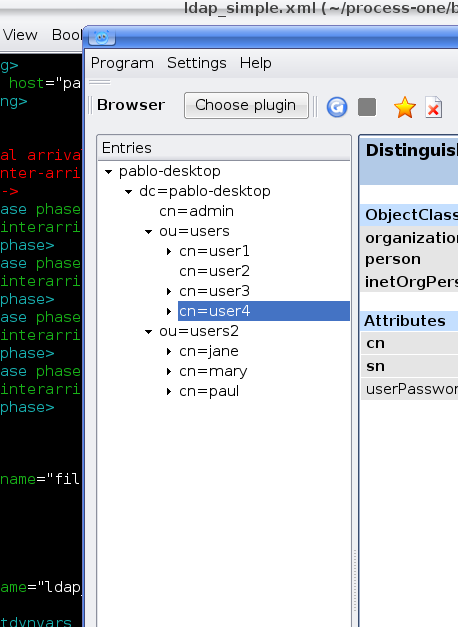
\includegraphics[width=0.4\linewidth]{ldap-hierarchy}
    \end{center}
      \caption{LDAP Hierarchy}
    \label{fig:ldap:hierarchy}
\end{figure}

the repository has users in two organizational units
\begin{enumerate}
\item users (with four members)
\item users2 (with tree members)
\end{enumerate}

For simplicity we set the password of each user to be  the same as its common name (cn).
Tsung Setup
We will use a CSV file as input, containing the user:password pairs
for our test. So we start by writing it, in this case we name the file \file{users.csv}

\begin{Verbatim}
user1;user1
user2;user2
user3;user3
user4;user4
jane;jane
mary;mary
paul;pablo
paul;paul
\end{Verbatim}

(the pair paul:pablo should fail to authenticate, we will note that in the Tsung report)
Then, in our Tsung scenario, we let Tsung know about this file

\begin{Verbatim}
    <options>
       <option name="file_server" id="users" value="users.csv"/>
    </options>
We use two dynamic variables to hold the username and password
    <setdynvars sourcetype="file" fileid="users" delimiter=";" order="iter">
               <var name="username" />
               <var name="password" />
     </setdynvars>
\end{Verbatim}

To start the authentication process we instruct Tsung to perform a search, to find the distinguished name of the user we are trying to authenticate

\begin{Verbatim}
  <ldap type="search" base="dc=pablo-desktop" filter="(cn=%%_username%%)"
        result_var="search_result" scope="wholeSubtree"></ldap>
\end{Verbatim}

As we need to access the search result, we specify it using the \varname{result\_var} attribute. This attribute tells Tsung in which dynamic variable we want to store the result (if the \varname{result\_var} attribute isn't set, Tsung doesn't store the search result in any place).
Finally,  we try to bind as that user.
\begin{Verbatim}
<request subst="true">
<ldap type="bind" user="%%ldap_auth:user_dn%%"
      password="%%_password%%"></ldap>
</request>
\end{Verbatim}
The only thing that remains to do is to implement the \varname{ldap\_auth:user\_dn} function, that extract the distinguished name from the search result.

\begin{Verbatim}
-module(ldap_auth).
-export([user_dn/1]).
user_dn({_Pid,DynVars}) ->
      [SearchResultEntry] = proplists:get_value(search_result,DynVars),
      {_,DN,_} = SearchResultEntry,
      DN.
\end{Verbatim}

We aren't covering errors here. supposing that there is always one (and only one) user found, that we extract from the \varname{search\_result} variable (as defined in the previous search operation).
Each entry in the result set is a SearchResultEntry record. The record definition can be found in \file{<TSUNG_DIR>/include/ELDAPv3.hrl}.

As we only need to access the distinguished name of the object, we index into the result tuple directly. But if you need to access other attributes you probably will want to include the appropriate .hrl and use the record syntax instead. One of the eight user:password pairs in our users file was wrong, so we expect 1/8 of the authentication attempts to fail.

Indeed, after running the scenario we can confirm this in the Tsung
report (see figure \ref{fig:ldap:results}). The bind operation maintains two
counters: \varname{ldap\_bind\_ok} and \varname{ldap\_bind\_error},
that counts successful and unsuccessful bind attempts.

\begin{figure}[htb]
  \begin{center}
    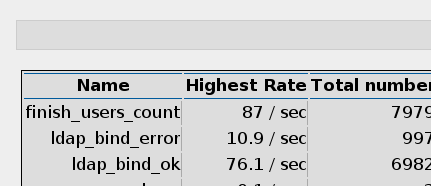
\includegraphics[width=0.4\linewidth]{ldap-results}
    \end{center}
      \caption{LDAP Results}
    \label{fig:ldap:results}
\end{figure}

\paragraph{Other examples}

\begin{Verbatim}
<session probability="100" name="ldap-example" type="ts_ldap">
  <request>
     <ldap type="bind" user="uid=foo" password="bar"/>
  </request>

   <request>
       <ldap type="search" base="dc=pablo-desktop" filter="(cn=user2)"
       scope="wholeSubtree"></ldap>
   </request>

<!-- Add. Adds a new entry to the directory* -->
  <request subst="true">
  <ldap type="add" dn="%%_new_user_dn%%" >
   <attr type="objectClass">
    <value>organizationalPerson</value>
    <value>inetOrgPerson</value>
    <value>person</value>
   </attr>
   <attr type="cn"><value>%%_new_user_cn%%</value></attr>
   <attr type="sn"><value>fffs</value></attr>
 </ldap>
</request>

<!-- Modify. Modifies an existing entry; type=add|delete|modify-->
 <request subst="false">
   <ldap type="modify" dn="cn=u119843,dc=pablo-desktop" >
    <modification type="replace">
     <attr type="sn"><value>SomeSN</value></attr>
     <attr type="mail"><value>some@mail.com</value></attr>
    </modification>
  </ldap>
 </request>
</session>
\end{Verbatim}

\subsection{Advanced features}

\subsubsection{Dynamic substitutions}

 Dynamic substitution are mark-up placed in element of the scenario.
For HTTP, this mark-up can be placed in basic authentication (www\_authenticate
tag: userid and passwd attributes), URL (to change GET parameter)
and POST content.

Those mark-up are of the form \userinput{\%\%Module:Function\%\%}.
Substitutions are executed on a request-by-request basis, only if the
request tag has the attribute \userinput{subst="true"}.

When a substitution is requested, the substitution mark-up is replaced by
the result of the call to the Erlang function:
\userinput{Module:Function(\{Pid, DynData\})} where Pid is the Erlang process
id of the current virtual user and DynData the list of all Dynamic
variables (\strong{Warn: before version 1.1.0, the argument was just the
  Pid !}).

Here is an example of use of substitution in a Tsung scenario:

\begin{Verbatim}
<session name="rec20040316-08:47" probability="100" type="ts_http">
 <request subst="true">
  <http url="/echo?symbol=%%symbol:new%%" method="GET">
  </http></request>
</session>
\end{Verbatim}

Here is the Erlang code of the module used for dynamic substitution:

\begin{Verbatim}
-module(symbol).
-export([new/1]).

new({Pid, DynData}) ->
    case random:uniform(3) of
        1 -> "IBM";
        2 -> "MSFT";
        3 -> "RHAT"
    end.
\end{Verbatim}

(use \command{erlc} to compiled the code, and put the resulting .beam
file in \file{\$PREFIX/lib/erlang/lib/tsung-X.X.X/ebin/} on all client
machines)

As you can see, writing scenario with dynamic substitution is trivial.

If you want to set unique id, you can use the built-in function
\varname{ts\_user\_server:get\_unique\_id}.
\begin{Verbatim}
<session name="rec20040316-08:47" probability="100" type="ts_http">
 <request subst="true">
  <http url="/echo?id=%%ts_user_server:get_unique_id%%" method="GET">
  </http></request>
</session>
\end{Verbatim}

\subsubsection{Reading external file}
\strong{New in 1.0.3}: A new  module \varname{ts\_file\_server} is available. You
can use it to read external files. For example, if you need to read user
names and passwd from a CSV file, you can do it with it (currently,
you can read only a single file). \emph{Note: Reading usernames and
password from a CSV file is not possible for Jabber.}

You have to add this in the XML configuration file:
\begin{Verbatim}
 <option name="file_server"  value="/tmp/userlist.csv"></option>
\end{Verbatim}

\strong{New in 1.2.2}: You can read several files, using the \varname{id}
attribute to identify each file:
\begin{Verbatim}
 <option name="file_server"  value="/tmp/userlist.csv"></option>
 <option name="file_server" id='random' value="/tmp/randomnumbers.csv"></option>
\end{Verbatim}

Now you can build you own function to use it, for example, create a
file called \file{readcsv.erl}:

\begin{Verbatim}
-module(readcsv).
-export([user/1]).

user({Pid,DynVar})->
    {ok,Line} = ts_file_server:get_next_line(),
    [Username, Passwd] = string:tokens(Line,";"),
    "username=" ++ Username ++"&password=" ++ Passwd.
\end{Verbatim}

The output of the function will be a string \userinput{username=USER\&password=PASSWORD}

Then compile it with \command{erlc readcsv.erl} and put
\file{readcsv.beam} in \file{\$prefix/lib/erlang/lib/tsung-VERSION/ebin} directory.

(If the file has an id set to \userinput{random}, change the call to: \texttt{ts\_file\_server:get\_next\_line(random)}.)

Then use something like this in your session:

\begin{Verbatim}
  <request subst="true">
    <http url='/login.cgi' version='1.0' contents='%%readcsv:user%%&amp;op=login'
    content_type='application/x-www-form-urlencoded' method='POST'>
    </http>
  </request>
\end{Verbatim}

Two functions are available: \varname{ts\_file\_server:get\_next\_line}
and \varname{ts\_file\_server:get\_random\_line}. For the
\varname{get\_next\_line} function, when the end of file is reached, the
first line of the file will be the next line.

\strong{New in 1.3.0}: you no longer have to create an external
function to parse a simple csv file: you can use \varname{setdynvars}
(see next section for detailed documentation):

\begin{Verbatim}
<setdynvars sourcetype="file" fileid="userlist.csv" delimiter=";" order="iter">
 <var name="username" />
 <var name="user_password" />
</setdynvars>
\end{Verbatim}

This defines two dynamic variables \varname{username} and
\varname{user\_password} filled with the next entry from the csv
file. Using the previous example, the request is now:
\begin{Verbatim}
  <request subst="true">
    <http url='/login.cgi' version='1.0'
      contents='username=%%_username%%&amp;password=%%_user_password%%&amp;op=login'
    content_type='application/x-www-form-urlencoded' method='POST'>
    </http>
  </request>
\end{Verbatim}

Much simpler than the old method !

\subsubsection{Dynamic variables}

In some cases, you may want to use a value given by the server in a
response later in the session, and this value is \strong{dynamically
generated} by the server for each user. For this, you can use
\userinput{<dyn\_variable>} in the scenario

Let's take an example with HTTP. You can easily grab a value in a HTML
form like:
\begin{Verbatim}
<form action="go.cgi" method="POST">
<hidden name="random_num" value="42"></form>
</form>
\end{Verbatim}

with:
\begin{Verbatim}
 <request>
   <dyn_variable name="random_num" ></dyn_variable>
   <http url="/testtsung.html" method="GET" version="1.0"></http>
 </request>
\end{Verbatim}

Now \varname{random\_num} will be set to 42 during the user's session. It's
value will be replace in all mark-up of the form
\userinput{\%\%\_random\_num\%\%} if and only if the \varname{request} tag has the
attribute \userinput{subst="true"}, like:

\begin{Verbatim}
    <request subst="true">
      <http url='/go.cgi' version='1.0'
      contents='username=nic&amp;random_num=%%_random_num%%&amp;op=login'
      content_type='application/x-www-form-urlencoded' method='POST'>
      </http>
    </request>
\end{Verbatim}

If the dynamic value is not a form variable, you can set a regexp by
hand, for example to get the title of a HTML page:
\begin{Verbatim}
    <request>
      <dyn_variable name="mytitlevar"
                    regexp="&lt;title&gt;\(.*\)&lt;/title&gt;"/>
      <http url="/testtsung.html" method="GET" version="1.0"></http>
    </request>
\end{Verbatim}

\strong{Since version 1.3.0}, more powerful dynamic variables are implemented:

You can set dynamic variables not only while parsing server data, but
you can build them using external files or generated them with a function
or generate random numbers/strings:

Five type of dynamic variables are currently implemented (\varname{sourcetype} tag):
\begin{enumerate}
\item Dynamic variables defined by calling an erlang function:
\begin{Verbatim}
      <setdynvars sourcetype="erlang" callback="ts_user_server:get_unique_id">
        <var name="id1" />
      </setdynvars>
\end{Verbatim}
\item Dynamic variables defined by parsing an external file:
\begin{Verbatim}
      <setdynvars sourcetype="file" fileid="userdb" delimiter=";" order="iter">
        <var name="user" />
        <var name="user_password" />
      </setdynvars>
\end{Verbatim}
\varname{delimiter} can be any string, and \varname{order} can be
\userinput{iter} or \userinput{random}
\item Dynamic variable can a random number
\begin{Verbatim}
      <setdynvars sourcetype="random_number" start="3" end="32">
        <var name="rndint" />
      </setdynvars>
\end{Verbatim}
\item Dynamic variable can a random string
\begin{Verbatim}
      <setdynvars sourcetype="random_string" length="13">
        <var name="rndstring1" />
      </setdynvars>
\end{Verbatim}
\item Dynamic variable can a urandom string: this is much faster than
  the random string, but the string is not really random: the same set
  of character is always used.
\end{enumerate}

A \varname{setdynvars} can be defined anywhere in a session.

\subsubsection{Checking the server's response}

\paragraph{Regexp}

With the tag \varname{match} in a \varname{request} tag, you can check
the server's response against a given string, and do some actions
depending on the result. In any case, if it matches, this will
increment the \varname{match} counter, if it does not match, the
\varname{nomatch} counter will be incremented.

For example, let's say you want to test a login page. If the login is
ok, the server will respond with \computeroutput{Welcome !} in the
HTML body, otherwise not. To check that:
\begin{Verbatim}
 <request>
      <match do="continue" when="match">Welcome !</match>
      <http url='/login.php' version='1.0' method='POST'
       contents='username=nic&amp;user_password=sesame'
       content_type='application/x-www-form-urlencoded' >
 </request>
\end{Verbatim}

You can use a regexp instead of a simple string.

The list of available actions to do is:
\begin{itemize}
\item continue
\item abort : abort the session
\item restart: restart the session. The maximum number of
  restarts is 3 by default.
\item loop: repeat the request, after 5 seconds. The maximum number of
  loops is 20 by default.
\end{itemize}

You can mixed several match tag in a single request:
\begin{Verbatim}
 <request>
      <match do="loop" sleep_loop="5" max_loop="10" when="match">Retry</match>
      <match do="abort" when="match">Error</match>
      <http url='/index.php' method=GET'>
 </request>
\end{Verbatim}

You can also do the action on "nomatch" instead of "match".

\paragraph{XPath}

A new way to analyze the server response has been introduced in the
release \strong{1.3.0}. It is only for the HTTP plugin since it is
based on XML/HTML parsing. This feature uses the mochiweb library
and \strong{only works with erlang R12B and newer version}.

This give us some benefices:

\begin{itemize}
\item XPath is simple to write and to read, and match very well with
  html pages
\item The parser works on binaries(), and doesn't create any
  string(). In constrant, the regexp module works on string(), so the
  entire page needs to be \varname{binary\_to\_list/1} transformed before
  processing it.
\item The cost of parsing the html and build the tree is amortized
  between all the dyn\_variables defined for a given request
\end{itemize}

To utilize xpath expression, use a \varname{xpath} attribute when
defining the dyn\_variable, instead of \varname{regexp}, like:
\begin{Verbatim}
<dyn_variable name="field1_value" xpath="//input[@name='field1']/@value"/>
<dyn_variable name="title" xpath="/html/head/title/text()"/>
\end{Verbatim}

There is a bug in the xpath engine, result nodes from "descendant-or-self" aren't returned in document order. This isn't a problem for the most common cases.
However, queries like \userinput{//img[1]/@src} are not recommended, as the order of the \userinput{<img>} elements returned from //img is not the expected.
The order is respected for paths without "descendant-or-self" axis, so this: \userinput{/html/body/div[2]/img[3]/@src} is interpreted as expected and can be safely used.

Basic tests shows a x4 improvement in speed over the \emph{regexp} implementation.

\subsubsection{Loops}

\strong{Since 1.3.0}, it's now possible to add conditional/unconditional loops in a session:

\paragraph{<for>}


Repeat the enclosing actions a fixed number of times. A dynamic
variable is used as counter, so the current iteration could be used in
requests. List of attributes:

\begin{description}
\item[from] Initial Value
\item[to]   Last value
\item[incr] Amount to increment in each iteration
\item[var]  Name of the variable to hold the counter
\end{description}

\begin{Verbatim}
 <for from="1" to="10" incr="1" var="counter">
  [...]
  <request> <http url="/page?id=%%_counter%%"></http> </request>
  [...]
 </for>
\end{Verbatim}

\paragraph{<repeat>}
Repeat the enclosing action (while|until) some condition. This is
intended to be used together with \userinput{dyn\_variable} declarations. List of
attributes:

\begin{description}
\item[name] Name of the repeat
\item[max\_repeat] Max number of loops
\end{description}

The last element of repeat must be either \userinput{<while>} or \userinput{<until>} example:
\begin{Verbatim}
  <repeat name="myloop" max_repeat="40">

   [...]

   <request>
     <dyn_variable name="result" regexp="Result: (.*)"/>
     <http url="/random" method="GET" version="1.1"></http>
   </request>

   [...]

  <until var="result" eq="5"/> </repeat>
\end{Verbatim}

\section{Statistics and reports}
\label{sec:statistics-reports}

\subsection{Available stats}

\begin{itemize}
\item  \varname{request} Response time for each request.
\item  \varname{page} Response time for each set of requests (a page is a group
  of request not separated by a thinktime).
\item  \varname{connect} Duration of the connection establishment.
\item  \varname{reconnect} number of reconnection.
\item  \varname{size\_rcv} Size of responses in bytes.
\item  \varname{size\_sent} Size of requests in bytes.
\item  \varname{session} Duration of a user's session.
\item  \varname{users} Number of simultaneous users.
\item  \varname{connected} Number of simultaneous connected users. \strong{new
  in 1.2.2}.
\item  custom transactions
\end{itemize}

The mean response time (for requests, page, etc.) is computed every 10
sec (and reset). That's why you have the highest mean and lowest mean
values in the Stats report. \strong{Since version 1.3.0}, the mean for
the whole test is also computed.

HTTP specific stats:
\begin{itemize}
\item counter for each response status (200, 404, etc.)
\end{itemize}

Jabber specific stats:
\begin{itemize}
\item \varname{request\_noack} Counter of \varname{no\_ack} requests. Since
  response time is meaningless with \varname{no\_ack}
  requests, we keep a separate stats for this. \strong{new in 1.2.2}.
\item \varname{bidi\_msg\_skip} Only if bidi is true for a
  session. counter the number of messages received from the server
  without doing anything.  \strong{new in 1.2.2}.
\item \varname{bidi\_msg\_sent} Only if bidi is true for a
  session. Count the number of messages sent to the server in response
  of a message received from from the server. \strong{new in 1.2.2}.
\end{itemize}

\subsection{Design}

A bit of explanation on the design and internals of the statistics engine:

Tsung was designed to handle thousands of requests/sec, for very
long period of times (several hours) so it do not write all data to
the disk (for performance reasons). Instead it computes on the fly an
estimation of the mean and standard variation for each type of data,
and writes these estimations every 10 seconds to the disk (and then
starts a new estimation for the next 10 sec). These computations are
done for two kinds of data:
\begin{itemize}
\item \varname{sample}, for things like response time
\item \varname{sample\_counter} when the input is a cumulative one (number of
packet sent for ex.).
\end{itemize}

There are also two other types of useful data (no averaging is done for
those) :
\begin{itemize}
\item \varname{counter}: a simple counter, for HTTP status code for ex.
\item \varname{sum} for ex. the cumulative HTTP response's size (it gives an
estimated bandwidth usage).
\end{itemize}



\subsection{Generating the report}

cd to the log directory of your test (say
\file{~/.tsung/log/20040325-16:33/}) and use the script
\command{tsung\_stats.pl}:

\begin{Verbatim}
/usr/lib/tsung/bin/tsung_stats.pl
\end{Verbatim}

\strong{You can generate the statistics even when the  test is running !}

use \userinput{--help} to view all available options:

\begin{Verbatim}
Available options:
        [--help] (this help text)
        [--verbose]
        [--debug]
        [--noplot]  (don't make graphics)
        [--gnuplot <command>]  (path to the gnuplot binary)
        [--nohtml]  (don't create HTML reports)
        [--logy]  (logarithmic scale for Y axis)
        [--tdir <template_dir>] (Path to the HTML tsung templates)
        [--noextra  (don't generate graphics from extra data (os monitor, etc)
        [--stats <file>] (stats file to analyse, default=tsung.log)
\end{Verbatim}

\subsection{Tsung summary}
Figure \ref{fig:report} show an example of a summary report.
\begin{figure}[htb]
  \begin{center}
    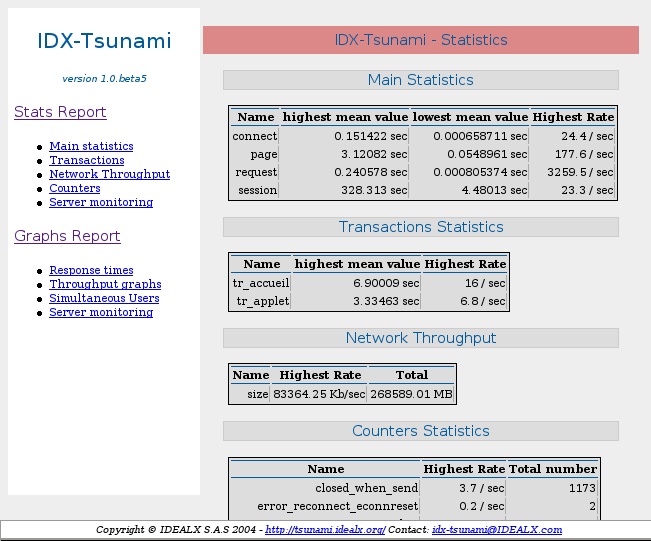
\includegraphics[width=0.6\linewidth]{tsung-report}
    \end{center}
      \caption{Report}
    \label{fig:report}
\end{figure}

\subsection{Graphical overview}

Figure \ref{fig:graph} show an example of a graphical report.

\begin{figure}[htb]
  \begin{center}
    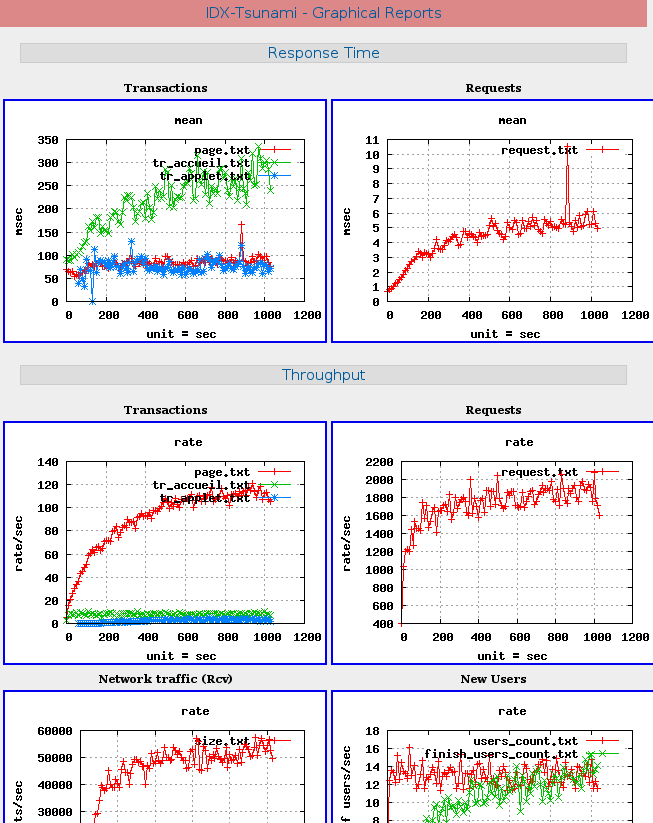
\includegraphics[width=0.6\linewidth]{tsung-graph}
    \end{center}
      \caption{Graphical output}
    \label{fig:graph}
\end{figure}

\section{References}

\begin{itemize}
\item \program{Tsung} home page: \url{http://tsung.erlang-projects.org/}
\item \program{Tsung} description (French)\footnote{\url{http://www.erlang-projects.org/Members/mremond/events/dossier_de_presentat/block_10766817551485/file}}
\item Erlang web site \url{http://www.erlang.org/}
\item Erlang programmation, Mickaël Rémond, Editions Eyrolles, 2003
  \footnote{\url{http://www.editions-eyrolles.com/php.accueil/Ouvrages/ouvrage.php3?ouv_ean13=9782212110791}}
\item \emph{Making reliable system in presence of software errors}, Doctoral Thesis,
Joe Armstrong, Stockholm, 2003 \footnote{\url{http://www.sics.se/~joe/thesis/armstrong_thesis_2003.pdf}}
\item \emph{Tutorial on How to write a Tsung plugin}, written by t ty, \url{http://www.process-one.net/en/wiki/Writing_a_Tsung_plugin/}
\end{itemize}

\section{Acknowledgments}

The first version of this document was based on a talk given by Mickael
Rémond\footnote{\email{mickael.remond@erlang-fr.org}} during an Object
Web benchmarking workshop in April 2004 (more info at
\url{http://jmob.objectweb.org/}).


\begin{appendix}

\section{Frequently Asked Questions}

\subsection{Tsung crashes when I start it }

Does your Erlang system has ssl support enabled ?

to test it:
\begin{Verbatim}
  > erl
  Eshell V5.2  (abort with ^G)
  1> ssl:start().
  you should see 'ok'
\end{Verbatim}

\subsection{Tsung still doesn't start ...}

Most of the time, when a crash happened at startup without any traffic
generated, the problem arise because the main Erlang controller node cannot
create a "slave" Erlang virtual machine. The message looks like:

\begin{Verbatim}
===============================================
=ERROR REPORT==== 4-May-2004::22:38:26 ===
** Generic server ts_config_server terminating
** Last message in was {'$gen_cast',{newbeam,myshortname,[]}}
** When Server state == {state,{config,
                                     undefined,
                                     5,
                                     full,
                                     undefined,
                                     [{client,
                                          "myshortname",
                                          2.00000,
                                          5,
                                          [{10,68,133,140}]}],
                                     {server,"foo.net",80,gen_tcp},
                                     [],
                                     [{arrivalphase,
                                          1,
                                          60,
                                          undefined,
                                          undefined,
                                          5.00000e-5,
                                          infinity}],
                                     undefined,
                                     [{session,
                                          1,
                                          100,
                                          ts_http,
                                          parse,
                                          true,
                                          undefined}],
                                     14,
                                     3,
                                     7,
                                     6,
                                     "negociate"},
  "/home/username/.tsung/log/20040204-18:32",
                               undefined,
                               0,
                               undefined,
                               2.00000}
** Reason for termination ==
** {{badmatch,{error,timeout}},
    [{ts_config_server,handle_cast,2},
     {gen_server,handle_msg,6},
     {proc_lib,init_p,5}]}
\end{Verbatim}
%%%$

Tsung launches a new erl virtual machine to do the actual
injection even when you have only one machine in the injection
cluster. This is because it needs to by-pass some limit with the number
of open socket from a single process (1024 most of the time). The idea
is to have several system processes (Erl beam) that can handle only a
small part of the network connection from the given computer. When the
\varname{maxclient} limit (simultaneous) is reach, a new Erlang beam is launched
and the newest connection can be handled by the new beam).

The problem is that the Erlang slave module cannot start a local slave
node. It tries to start it with the short node name
\varname{"myshortname"} (\command{erl -sname myshortname}).
 If this fails the injection process cannot
start. Most of the time, adding the short name with the correct IP
address in the \file{/etc/hosts} file is sufficient to make it work.

You can test this using these simple commands:
\begin{Verbatim}
>erl -rsh ssh -sname foo -setcookie mycookie

Eshell V5.4.3 (abort with ^G)
(foo@myhostname)1>slave:start(remotehost,bar,"-setcookie mycookie").
\end{Verbatim}
You should see this: \computeroutput{\{ok,bar@remotehost\}}

If you got \computeroutput{\{error,timeout\}}, it probably comes from
a firewall dropping erlang packets; indeed erlang virtual machines use
several tcp ports (dynamically generated) to communicate.
The timeout can also comes from the use of SELinux. You should disable it.


Note that you do not need to use the 127.0.0.1 address in the configuration file.
It will not work if you use it as the injection interface. The shortname
of your client machine should not refer to this address.

\strong{New in 1.1.0}: If you don't use the distributed feature of
Tsung and have trouble to start a remote beam on a local machine,
you can set the \varname{'use\_controller\_vm'} attribute to true, for ex.:

\begin{Verbatim}
  <client host="mymachine" use_controller_vm="true">
\end{Verbatim}

You may also have problems due to the sshd configuration:

For example, for SuSE 9.2 sshd is compiled with restricted set of
paths (\ie{} when you shell into the account you get the users shell,
when you execute a command via ssh you don't) and this makes it
impossible to start an erlang node (if erlang is installed in
\file{/usr/local} for example).

Run:

\begin{Verbatim}
ssh myhostname erl
\end{Verbatim}

If the erlang shell doesn't start then check what paths sshd was compiled with
(in SuSE see \file{/etc/ssh/sshd_config}) and symlink from one of the approved paths
to the erlang executable (thanks to Gordon Guthrie for reporting this).

\subsection{Why do i have error\_connect\_emfile errors ?}
\label{sec:faq:emfile}
emfile error means : \emph{too many open files}

This happens usually when you set a high value for \varname{maxusers}
(\varname{in the <client>} section) (the default value is 800).


The errors means that you are running out of file descriptors; you
must check that \varname{maxusers} is less than the maximum number of
file descriptors per process in your system (see \command{ulimit -n})

You can either raise the limit of your operating system ( see
\file{/etc/security/limits.conf} for Linux ) or decrease \varname{maxusers}
(Tsung will have to start several virtual machine on the same host to
bypass the maxusers limit).

\subsection{Tsung still crashes/fails  when I start it !}
First look at the log file
\file{~/.tsung/log/XXX/tsung_controller@yourhostname'} to see
if there is a problem.

If the file is not created and a crashed dump file is present, maybe
you are using a binary installation of Tsung not compatible with the
version of erlang you used.

If you see nothing wrong, you can compile \program{Tsung} with full
debugging: recompile with \command{make debug} , and
don't forget to set the loglevel to "debug" in the XML file.

To start the debugger or see what happen, start \program{tsung} with the
\userinput{debug} argument instead of \userinput{start}. You will have
an erlang shell on the \varname{tsung\_controller} node. Use
\command{toolbar:start().} to launch the graphical tools provided by
Erlang.

\subsection{Can i dynamically follow redirect with HTTP ?}

If your HTTP server sends 30X responses (redirect) with dynamic URLs,
you can handle this situation using a dynamic variable:

\begin{Verbatim}
<request>
  <dyn_variable name="redirect" regexp="Location: \(http://.*\)\r"/>
  <http url="index.html" method="GET" ></http>
</request>

<request subst="true">
  <http url="%%_redirect%%" method="GET"></http>
</request>
\end{Verbatim}

You can even handle the case where the server use several redirections
successively using a repeat loop (this works only with version 1.3.0 and up):

\begin{Verbatim}
  <request>
    <dyn_variable name="redirect" regexp="Location: \(http://.*\)\r"/>
    <http url='/test/redirect.html' method='GET'></http>
  </request>

  <repeat name="redirect_loop" max_repeat="5">
    <request subst="true">
      <dyn_variable name="redirect" regexp="Location: \(http://.*\)\r"/>
      <http url="%%_redirect%%" method="GET"></http>
    </request>
    <until var="redirect" eq=""/>
  </repeat>
\end{Verbatim}

\subsection{What is the format of the stats file tsung.log ?}

\begin{Verbatim}
# stats: dump at 1218093520
stats: users 247 247
stats: connected 184 247
stats: users_count 184 247
stats: page 187 98.324 579.441 5465.940 2.177 9.237 595 58
stats: request 1869 0.371 0.422 5.20703125 0.115 0.431 7444062 581
stats: connect 186 0.427 0.184 4.47216796875 0.174 0.894 88665254 59
stats: tr_login 187 100.848 579.742 5470.223 2.231 56.970 91567888 58
stats: size_rcv 2715777 3568647
stats: 200 1869 2450
stats: size_sent 264167 347870
# stats: dump at 1218093530
stats: users 356 356
stats: users_count 109 356
stats: connected -32 215
stats: page 110 3.346 0.408 5465.940 2.177 77.234 724492 245
stats: request 1100 0.305 0.284 5.207 0.115 0.385 26785716 2450
stats: connect 110 0.320 0.065 4.472 0.174 0.540 39158164 245
stats: tr_login 110 3.419 0.414 5470.223 2.231 90.461 548628831 245
stats: size_rcv 1602039 5170686
stats: 200 1100 3550
stats: size_sent 150660 498530
 ...
\end{Verbatim}

 the format is, for \varname{request}, \varname{page},
 \varname{session} and transactions (\varname{tr\_XXX}:

 \texttt{ \# stats:'name' 10sec\_count, 10sec\_mean, 10sec\_stdvar,
   max, min, mean, count}

 or for HTTP returns code, size ...

\texttt{ \# stats:'name' count(during the last 10sec), totalcount(since the beginning)}

\subsection{How can I compute percentile/quartiles/median for transactions or requests
  response time ?}

It's not directly possible. But since \strong{version 1.3.0}, you can
use a new experimental statistic backend: set \userinput{backend="fullstats"}

This will print every statistics data in a raw format in a file named
\file{tsung-fullstats.log}. \strong{Warning}: this may impact the performance of
the controller node (a lot of data may be written to disk).

The data looks like:
\begin{Verbatim}
{sum,connected,1}
{sum,connected,-1}
[{sample,request,214.635},
 {sum,size_rcv,268},
 {sample,page,831.189},
 {count,200},
 {sum,size_sent,182},
 {sample,connect,184.787},
 {sample,request,220.974},
 {sum,size_rcv,785},
 {count,200},
 {sum,size_sent,164},
 {sample,connect,185.482}]
{sum,connected,1}
[{count,200},{sum,size_sent,161},{sample,connect,180.812}]
[{sum,size_rcv,524288},{sum,size_rcv,524288}]
\end{Verbatim}

You will have to write your own script to analyze the output.
The format of the file may change in a future release.


\subsection{How can I specify the number of concurrent users ?}

You can't. But it's on purpose: the load generated by
\program{Tsung} is dependent on the arrival time between new
clients. Indeed, once a client has finished his session in
\program{tsung}, it stops. So the number of concurrent users is
a function of the arrival rate and the mean session duration.

For example, if your web site has $1000$ visits/hour, the arrival rate
is $1000/3600 = 0.2778$ visits/second. If you want to simulate the same
load, set the inter-arrival time is to $1/0.27778 = 3.6 sec$ (\texttt{<users
interarrival="3.6" unit="second">} in the \varname{arrivalphase} node in the
XML config file).

\subsection{SNMP monitoring doesn't work ?!}

It use SNMP v1 and the 'public' community. It has been tested with
\url{http://net-snmp.sourceforge.net/}.

You can try with \command{snmpwalk} to see if your snmpd config is ok:

\begin{Verbatim}
>snmpwalk -v 1 -c public IP-OF-YOUR-SERVER .1.3.6.1.4.1.2021.4.5.0
UCD-SNMP-MIB::memTotalReal.0 = INTEGER: 1033436
\end{Verbatim}

SNMP doesn't work with erlang R10B and Tsung older than 1.2.0.

There is a small bug in the \file{snmp_mgr} module in old Erlang
release (R9C-0). You have to apply this patch to make it
work. This is fixed in erlang R9C-1 and up.


\begin{Verbatim}
--- lib/snmp-3.4/src/snmp_mgr.erl.orig  2004-03-22 15:21:59.000000000 +0100
+++ lib/snmp-3.4/src/snmp_mgr.erl       2004-03-22 15:23:46.000000000 +0100
@@ -296,6 +296,10 @@
     end;
 is_options_ok([{recbuf,Sz}|Opts]) when 0 < Sz, Sz =< 65535 ->
     is_options_ok(Opts);
+is_options_ok([{receive_type, msg}|Opts]) ->
+    is_options_ok(Opts);
+is_options_ok([{receive_type, pdu}|Opts]) ->
+    is_options_ok(Opts);
 is_options_ok([InvOpt|_]) ->
     {error,{invalid_option,InvOpt}};
 is_options_ok([]) -> true.
\end{Verbatim}

\section{Errors list}

\begin{description}
\item[error\_closed] Only for non persistent session (XMPP); the
  server unexpectedly closed the connection; the session is aborted.
\item[error\_inet\_<ERRORNAME>] Network error; see
  \url{http://www.erlang.org/doc/man/inet.html} for the list of all errors.
\item[error\_unknown\_data] Data received from the server during a
  thinktime (not for unparsed protocol like XMPP). The session is
  aborted.
\item[error\_unknown\_msg] Unknown message received (see the log
  files for more information). The session is aborted.
\item[error\_unknown] Abnormal termination of a session, see
  log file for more information.
\item[error\_repeat\_<REPEATNAME>] Error in a repeat loop (undefined
  dynamic variable usually).
\item[error\_send\_<ERRORNAME>] Error while sending data to the
  server, see  \url{http://www.erlang.org/doc/man/inet.html} for the list of all errors.
\item[error\_send] Unexpected error while sending data to the server,
  see the logfiles for more information.
\item[error\_connect\_<ERRORNAME>] Error while establishing a
  connection to the server.  See  \url{http://www.erlang.org/doc/man/inet.html} for the list of all errors.
\item[error\_no\_online jabber] XMPP: No online user available (usually for a
  chat message destinated to a online user)
\item[error\_no\_offline jabber] XMPP: No offline user available (usually for a
  chat message destinated to a offline user)
\item[error\_no\_free\_userid] For XMPP: all users Id are already used
  (\varname{userid\_max} is too low ?)
\item[error\_next\_session] A clients fails to gets its session
  parameter from the config\_server; the controller may be overloaded ?
\item[error\_mysql\_<ERRNO>] Error reported by the mysql server (see \url{http://dev.mysql.com/doc/refman/5.0/en/error-messages-server.html})
\item[error\_mysql\_badpacket] Bad packet received for mysql server while parsing data.
\item[error\_pgsql] Error reported by the postgresql server.
\end{description}

\section{CHANGELOG}
\fvset{numbers=none,frame=lines,fontsize=\scriptsize,fontfamily=courier,fontshape=sl}
\VerbatimInput{../CHANGES}
\end{appendix}

\end{document}


%%% for AucTex/Emacs :
%%% Local Variables:
%%% eval:(setenv "TEXINPUTS" ":.:~/cvs/projetdoc//common/styles:./images:./figures:")
%%% mode: latex
%%% End:
